\newpage
\section{Auswertung}

    \subsection{Kontrastbestimmung}
        Die Messungen des Kontrasts ergeben, wie in \autoref{fig:Kontrast} zu sehen, zwei Maxima im zu erwartenden Bereich von circa 45° und 135°.
        
        \FloatBarrier

        \begin{figure}[h]
          \centering
          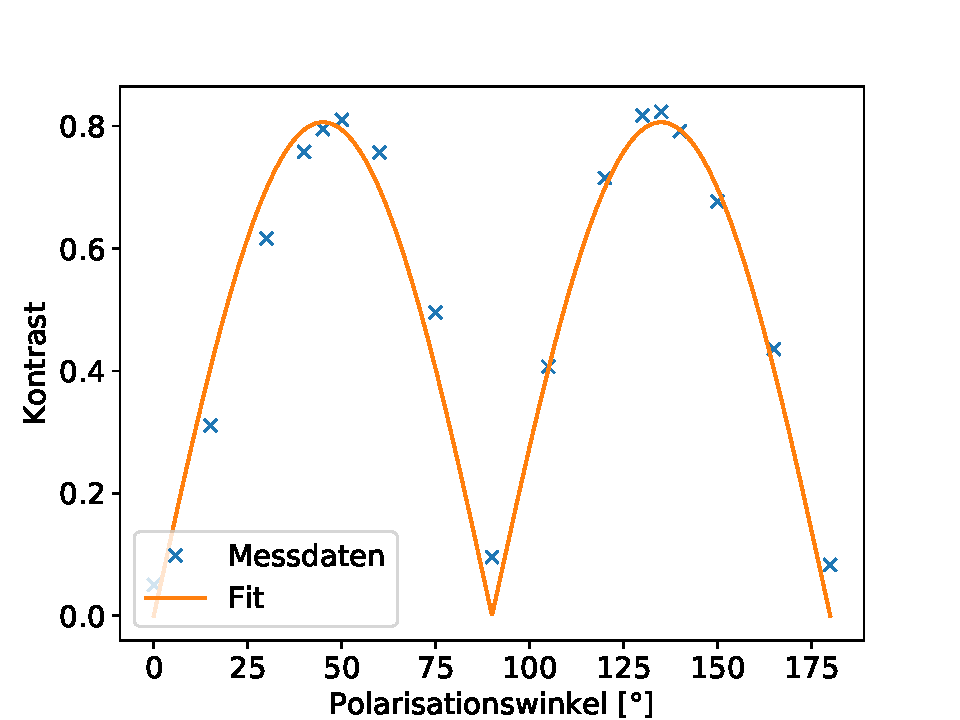
\includegraphics[width = 0.6\textwidth]{pictures/Kontrast.pdf}
          \caption{In der Grafik ist der gemessene Kontrast in Abhängigkeit des Polarisationswinkels des ins Interferometer einfallenden Lichtes aufgetragen.}
          \label{fig:Kontrast}
        \end{figure}

        \FloatBarrier

        Das absolute Maximum liegt mit \num{0.82} bei einem Polarisationswinkel von 135°, welcher demnach für die weiteren Messungen beibehalten wird.



    \subsection{Brechungsindex von Glas}
        Der Mittelwert der Nulldurchgänge aus den 10 aufgenommenen Messreihen \autoref{tab:Nullen_Glas} ergibt sich zu $\overline{\text{M}} = \num{33.40 +- 0.22}$ und entspricht auch dem Mittelwert der Maxima.
        Wenn $\overline{\text{M}}$ in \eqref{eqn:n_platte} eingesetzt wird, lässt sich der Brechungsindex von Glas direkt berechnen:

        \begin{equation}
            \text{n}_{\text{Glas}} = \num{1.53 +- 0.01}
        \end{equation}

        Zum Vergleich wird angenommen, dass Quarzglasplättchen genutzt werden. In diesem Fall lässt sich die Abweichung zum Theoriewert von $\text{n}_{\text{Glas, Theo}}=$\num{1.46}\cite{theeten_new_1978} zu

        \begin{equation*}
            A= \left|\frac{\text{n}_{\text{Glas}} - \text{n}_{\text{Glas, Theo}}}{\text{n}_{\text{Glas, Theo}}}\right| \approx (5,1 \pm 0,4) \%
        \end{equation*}

        bestimmen.


    \subsection{Brechungsindex von Luft}
        Bei den Messungen zur Bestimmung des Brechungsindizes von Luft, sind alle drei Messreihen exakt identisch, sodass sie nicht gemittelt werden müssen (siehe Tab.~\ref{tab:Nullen_Luft}). Aus der Zahl der Maxima, die der Zahl der 
        Nulldurchgänge entspricht, lässt sich anhand von \eqref{eqn:n_gas} und bekannten Parametern des Experiments, wie der Länge der Gaszelle und der Wellenlänge des Lasers, der zugehörige Brechungsindex
        bei entsprechendem Druck berechnen. Wenn das Quadrat des Brechungsindex n² gegen den Druck p in der Gaszelle aufgetragen wird, ergibt sich ein linearer Zusammenhang, der dem quadrierten Lorentz-Lorenz-Gesetz entspricht und neben dem Druck und des Brechungsindex auch die Temperatur zur Zeit der Messung $\text{T}_{\text{M}}=\SI{295.05}{\kelvin}$ und die allgemeine Gaskonstante R enthält. 


        \FloatBarrier

        \begin{figure}[h]
          \centering
          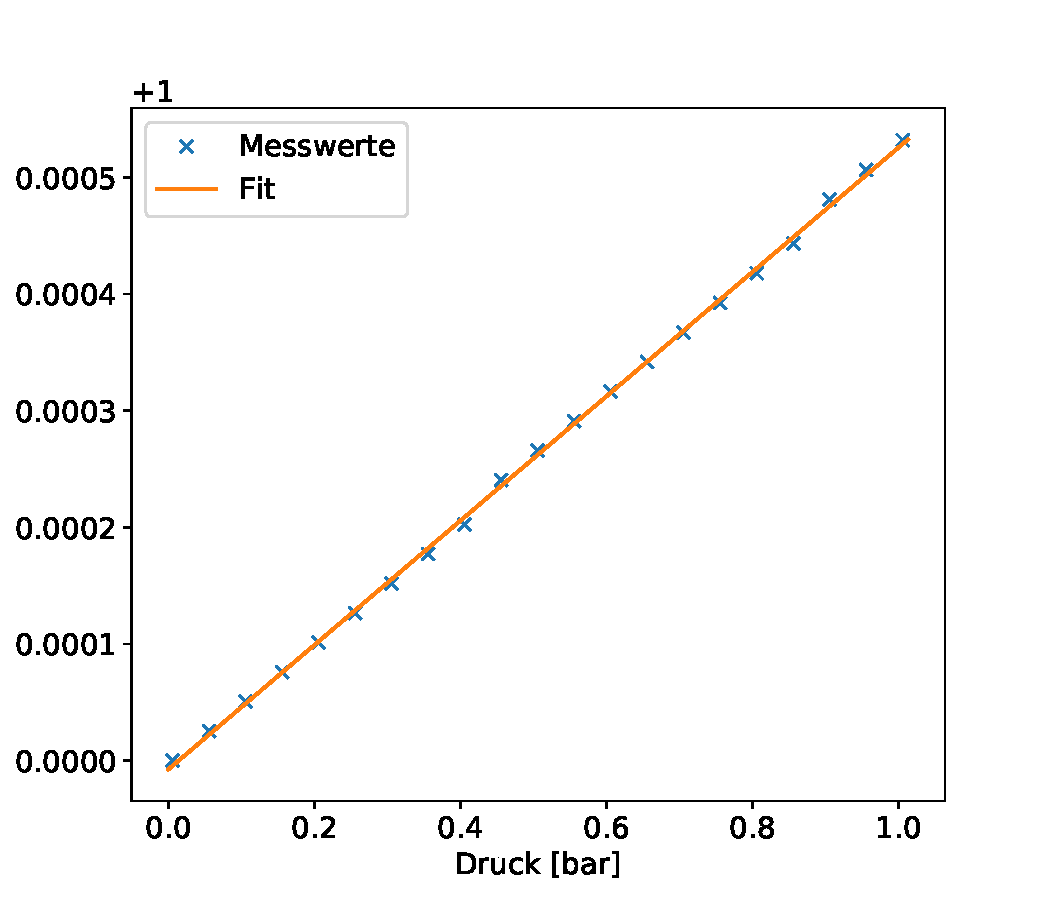
\includegraphics[width = 0.6\textwidth]{pictures/n_quad_fit.pdf}
          \caption{In der Grafik ist der lineare Zusammenhang zwischen dem Quadrat des Brechungsindex und dem Druck der Luft klar zu erkennen. Dieser wird auch linear regressiert, um die Molrefraktion A zu bestimmen.}
          \label{fig:n_quad_fit}
        \end{figure}

        \FloatBarrier

        \begin{align}
            \text{n}^2 &= \frac{3\text{A}}{\text{RT}_{\text{M}}} \cdot \text{p} + 1 \\
            \text{n}^2 &= \text{m} \cdot \text{p} + b
        \end{align}

        Aus der Steigung des linearen Zusammenhangs lässt sich die Molrefraktion A berechnen

        \begin{equation}
            \text{A} = \frac{\text{RT}_{\text{M}}\text{m}}{3} \qquad \text{mit} \qquad \text{m}=\SI{0.0005331(28)}{\per\bar}.
        \end{equation}

        Mit der nun bekannten Molrefraktion A lässt sich der Brechungsindex von Luft bei Normalbedingungen direkt über das nicht quadrierte Lorentz-Lorenz-Gesetz \eqref{eqn:lorentz} bestimmen:

        \begin{equation}
            \text{n}_{\text{Luft}}(\SI{1013}{\milli\bar}, \, \SI{288.15}{\kelvin}) = \num{1.0002764 +- 0.0000014}
        \end{equation}

        Damit liegt der Theoriewert von \num{1.00027653}~\cite{ciddor_refractive_1996} im Unsicherheitsintervall des bestimmten Brechungsindex bei Normalbedingungen. Die Nachkommastellen des bestimmten 
        Brechungsindex weichen um \num{0.0(5)}\% von denen des Theoriewerts ab.
        
